
%
% state - mapping stack
%

\section{Clustering implementations in Web Mapping}

Clustering in web mapping affects the way how vector data is processed and represented to the user.  According to the web mapping stack described in \ref{chapter:web-mapping-stack} we can differentiate between client-side and server-side clustering. A server-side clustering implementation will cluster the data already before sending it over the network to the browser client. In a client-side clustering implementation, the client receives the unclustered data set from the server and clusters it on its own.

\textbf{Client-side vs. server-side clustering}

Client-side clustering is convenient because of several reasons. The clustering task can be abstracted from the server without the need to account for server-side implementation details. It also relieves the server from performing the clustering task which can positively influence scalability. Executing the clustering task on the client-side also allows for better interaction, the user may zoom into or expand clusters without the need for an additional request to the server. 

On the other hand, client-side clustering forces the server to deliver the entire data set. This also means that a bigger amount of data has to be transferred over the network. Subsequently, the client needs to cope with receiving the larger data set and takes over the burden of clustering the data.

\subsection{Client-side clustering in Web Mapping}

When clustering on the client-side, the JavaScript mapping library receives the entire, unclustered data set and executes a clustering algorithm before visualizing the data to the user.

\begin{itemize}

\item The \textbf{Leaflet.markercluster}\footnote{\url{https://github.com/Leaflet/Leaflet.markercluster/}} library provides animated marker clustering for the Leaflet javascript mapping library. It combines the \textit{agglomerative hierarchical clustering algorithm} with a \textit{distance grid} (see chapters \ref{chapter:clustering-hierarchical} and \ref{chapter:clustering-grid}). The library features advanced cluster visualization techniques for representing shapes of clustered items and animations. When the user changes zooms into the map, clusters get expanded in a visual way and they collapse in the opposite direction.

Leaflet.markercluster leverages the advantages of being a client-side implementation by implementing a \textit{hierarchical clustering} approach that precalculates the clusters for all zoom levels. The markers are inserted into a distance grid on the lowest zoom level. The grid is then used to check for overlapping neighbors. If the inserted marker needs to get merged, this information is automatically propagated to upper levels within the hierarchy. Otherwise, the same checking procedure will be repeated for the inserted marker on the next, upper level.

The cluster visualization of Leaflet.markercluster is supported by the \textit{QuickHull}\footnote{\url{http://en.wikipedia.org/wiki/QuickHull/}} algorithm to compute the enclosing \textit{convex hull} of the clustered points as illustrated in b) in figure \ref{fig:leaflet}. In addition, a \textit{spiderfier} algorithm allows the user to select clustered points, even if they are positioned very closely to each other, see a) in figure \ref{fig:leaflet}.

The clustering task is computed in \textit{linear time} to the number of markers $n$ and the usually constant number of zoom levels. 

\begin{figure}[h]
  \begin{center}
    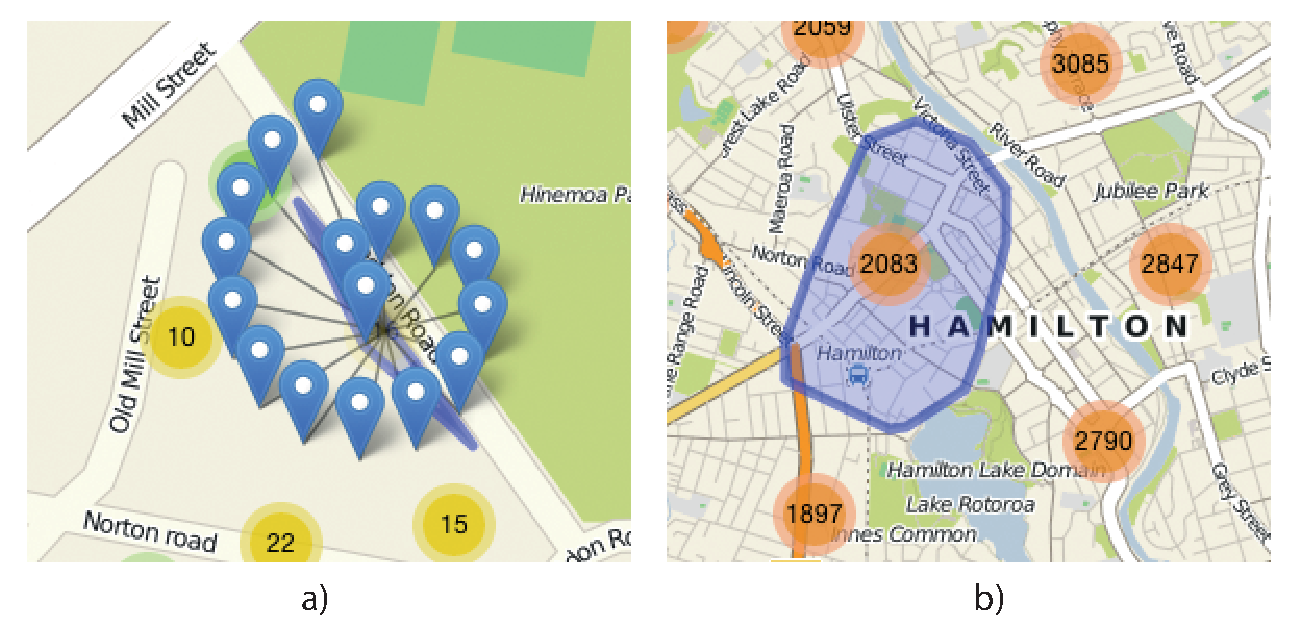
\includegraphics[width=1\textwidth]{figures/leaflet.pdf}
    \caption{Two screenshots taken from the Leaflet.markercluster example map: a) spiderfied representation to select from multiple overlapping points and b) the visualized convex hull of a cluster indicates the real shape of the cluster on mouse-hover.}
    \label{fig:leaflet}
  \end{center}
\end{figure}

\item The \textbf{OpenLayers Cluster Strategy}\footnote{\url{http://dev.openlayers.org/releases/OpenLayers-2.12/lib/OpenLayers/Strategy/Cluster.js}} is included in the OpenLayers library and provides a simple \textit{distance-based} client-side clustering.

When creating the clustering, the features are sequentially inserted. Every new feature is compared against all existing clusters. If the new feature overlaps with any cluster, it will get merged into the existing cluster. Otherwise, the feature is inserted as its own cluster. Once the data, viewport or zoom level changes, the clustering process will be re-initiated. 

The sequential insertion and the comparison to all existing clusters leads to a \textit{factorial time complexity} of the algorithm. 

\item \textbf{k-means clustering}\footnote{\url{http://polymaps.org/ex/kmeans.js}} is a clustering library for the \textit{Polymaps} JavaScript mapping library. It leverages the k-means squared error algorithm discussed in chapter \ref{chapter:k-means} to create clusters in linear time. As discussed, the k-means algorithm computes in \textit{linear time}.

\end{itemize}

Other client-side clustering libraries evaluated can be classified similarly to the previously discussed ones. Grid-based approaches similar to Leaflet.markercluster include the Clustr library\footnote{\url{https://github.com/mapbox/clustr}} for Modest Maps and Clusterer2\footnote{\url{http://www.acme.com/javascript/\#Clusterer}} for Google Maps. MarkerClustererPlus for Google Maps V3\footnote{\url{http://code.google.com/p/google-maps-utility-library-v3/wiki/Libraries\#MarkerClusterer}} takes an approach similar to the OpenLayers Cluster Strategy.

TODO: conclusion

\subsection{Server-side clustering in Web Mapping}

Server-side implementations cluster the data already before sending it over the network to the client.

While client-side clustering solutions are standardized towards available JavaScript mapping libraries, this doesn't apply to server-side implementations. Clustering on the server-side can be performed both on the database and/or application layer. The wide variety of tools involved in the server-side mapping stack from different spatial databases and programming languages seems to make it harder to establish off-the-shelf libraries for server-side clustering, as they always need to be integrates into an architecture specific to the use case.

\begin{itemize}

\item \textbf{Clustering maps} by Wannes Meert is the only scientific publication found that explores server-side clustering for web mapping. The study compares strengths and weaknesses of three different approaches (\textit{K-means}, \textit{Hierarichal clustering} and \textit{DBSCAN}) and finally implements density-based clustering. The solution is based on the \textit{DBSCAN} algorithm and uses the \text{R-tree} as indexing structure to speed up neighborhood searches. It is implemented and documented as a \textit{PHP server-side script}. The time complexity of the implemented and discussed final algorithm is quasilinear: $\BigO{n \log{n}}$ and the demonstration page\footnote{\url{http://www.wannesm.be/maps/}} asserts a clustering time of $\sim 1$ second for only 525 points~\cite{Meert06clustermaps}.

\item \textbf{Google Maps Hacks: Tips and Tools for Geographic Searching and Remixing} is a book that contains a section \textit{Hack 69. Cluster Markers at High Zoom Levels} that discussed various approaches to server-side cluster markers for Google Maps. The chapter evaluates different approaches from a quadratic-time $\BigO{n^2}$ implementation of the \textit{k-means} algorithm over a even worse cubic-time $\BigO{n^3}$, \textit{hierarchical clustering} approach. Finally, a \textit{naive grid-based clustering} solution is developed and documented as a \textit{CGI Perl Script} which is stated to perform in linear time $\BigO{n}$~\cite{Gibson06Gmapshacks}.

\item \textbf{Geoclustering}\footnote{\url{https://github.com/ahtih/Geoclustering}} is a Drupal 6 module designed to ``scale to 100 000+ markers''. By maintaining a cluster tree in a separate database table, it essentially pre-calculates clusters. Similar to the grid-based clustering algorithm \textit{Sting} described in \ref{chapter:clustering-grid}, by shifting the clustering complexity to the calculation of the cluster tree, queries can be performed in constant time, only linear to the number of grids $\BigO{g}$. This speed improvement is reduces the possibilities of dynamic filtering to bounding-box filters only. Filters on other properties of the indexed data would need to be pre-calculated into a more complex or separate cluster trees.

\item \textbf{Clustering in Apache Solr} has been researched as well. Solr integrates Carrot2 as a document clustering engine\footnote{\url{http://searchhub.org/2009/09/28/solrs-new-clustering-capabilities/}}. Spatial clustering isn't supported out-of-the-box, a tutorial written in German documents the conceptual implementation of grid-based clustering in Solr\footnote{\url{http://blog.sybit.de/2010/11/geografische-suche-mit-solr/}}. As Geohash support has been added to Solr to support proximity searches~\cite{Smiley11geohash}, it could be used as well for spatially clustering data.  

\end{itemize}


Other server-side clustering implementations have been evaluated briefly:

On the \textbf{database-layer}, \textit{SQLDM - implementing k-means clustering using SQL} describes a linear-time implementation of the k-means clustering algorithm in \textit{MySQL}\cite{Simha07sqldm}.
 The \textit{PostGIS} spatial extension for the \textit{PostreSQL} database provides grid-based clustering via \textit{ST\_SnapToGrid}\footnote{\url{http://postgis.refractions.net/docs/ST_SnapToGrid.html}}. Also, a k-means module\footnote{\url{http://pgxn.org/dist/kmeans/doc/kmeans.html}} (also see \footnote{\url{http://gis.stackexchange.com/questions/11567/spatial-clustering-with-postgis}}) and documentation for clustering indices based on \textit{Geohash} \footnote{\url{http://workshops.opengeo.org/postgis-intro/clusterindex.html\#clustering-on-geohash}} for PostGIS exist.

Further, \textbf{application-layer} clustering implementations are grid- and distance-based clustering for Google Maps in PHP\footnote{\url{http://www.appelsiini.net/2008/11/introduction-to-marker-clustering-with-google-maps}}. Vizmo is a research project that developed a server-side clustering component in PHP, Symfony2 and MySQL, (TODO check if code is published yet)\footnote{\url{http://www.globalimpactstudy.org/wp-content/uploads/2011/12/vizmo-poster.pdf}}. Beyond the primary scope of PHP applications, a Flex-based clustering implementation has been developed for ArcGIS server\footnote{\url{http://thunderheadxpler.blogspot.co.at/2008/12/clustering-20k-map-points.html}}. ClusterPy\footnote{\url{http://www.rise-group.org/risem/clusterpy/index.html}} is a library of spatially constrained clustering algorithms in Python and SGCS\footnote{\url{http://cran.r-project.org/web/packages/SGCS/}} is a package to build graph based clustering summaries for spatial point patterns in R.





















